Pour la sélection des composants, en plus des éléments imposés par le projet, nous avons décidé d'utiliser une manette et de concevoir un modèle 3D de voiture.

\subsection{Choix de la manette}
Le choix de la manette s'est imposé en raison de sa précision supérieure par rapport à la télécommande. En effet, les deux gâchettes arrière ainsi que les joysticks émettent des valeurs comprises entre 0 et 255. Couplées aux signaux PWM, ces caractéristiques nous ont offert une précision accrue tant au niveau de la vitesse que des manœuvres.

Quant au code de la manette, nous avons initialement utilisé la bibliothèque de bas niveau evdev, qui utilise directement les fichiers en mode d'accès caractère associés à la manette. Toutefois, nous avons ultérieurement opté pour la bibliothèque SDL 2.0, plus haut niveau, rendant ainsi notre robot compatible avec toutes les manettes.

\subsection{Modèle 3D}
En ce qui concerne le choix du modèle 3D, il s'est principalement orienté vers des considérations esthétiques. Nous avons privilégié un modèle compact qui évoquerait une véritable voiture télécommandée. La base du modèle est une voiture issue du jeu vidéo Rocket League, qui a pour caractéristiques d'être haute et large, rendant le montage des composants internes moins laborieux.

Pour concevoir ce modèle 3D, nous avons modifié un fichier .stl préexistant de la voiture en utilisant le logiciel SolidWorks. Les roues ont été prises comme point de départ pour déterminer les dimensions globales de la voiture, garantissant ainsi une cohérence visuelle avec les garde-boue et les roues fictives de devant. 

En ce qui concerne les composants visibles, tels que le capteur de distance et l'écran LCD, nous avons créé des logements spécifiques dans la carrosserie. Ces logements ont été conçus pour offrir une intégration fluide et discrète, assurant que ces composants s'intègrent naturellement à la conception extérieure de la voiture. Des ajustements minutieux ont été apportés pour garantir la précision et la stabilité du montage, tout en préservant l'esthétique originale du modèle.

Simultanément, nous avons essayé d'enlever le maximum de matière à l'intérieur du modèle afin d'y intégrer les composants internes et de diminuer le temps d'impression. Des supports spécifiques ont été ajoutés pour maintenir en place l'ensemble des éléments électroniques tout en facilitant l'accès pour d'éventuelles réparations ou modifications.

\newpage

Après avoir effectué ces modifications et quelques vérifications sur les dimensions des composants, nous avons envoyé le fichier .stl modifié pour l'impression 3D du modèle final, aboutissant à une voiture télécommandée compacte, esthétique et fonctionnelle.

\bigbreak
\begin{figure}[h]
    \begin{minipage}[c]{.46\linewidth}
        \centering
        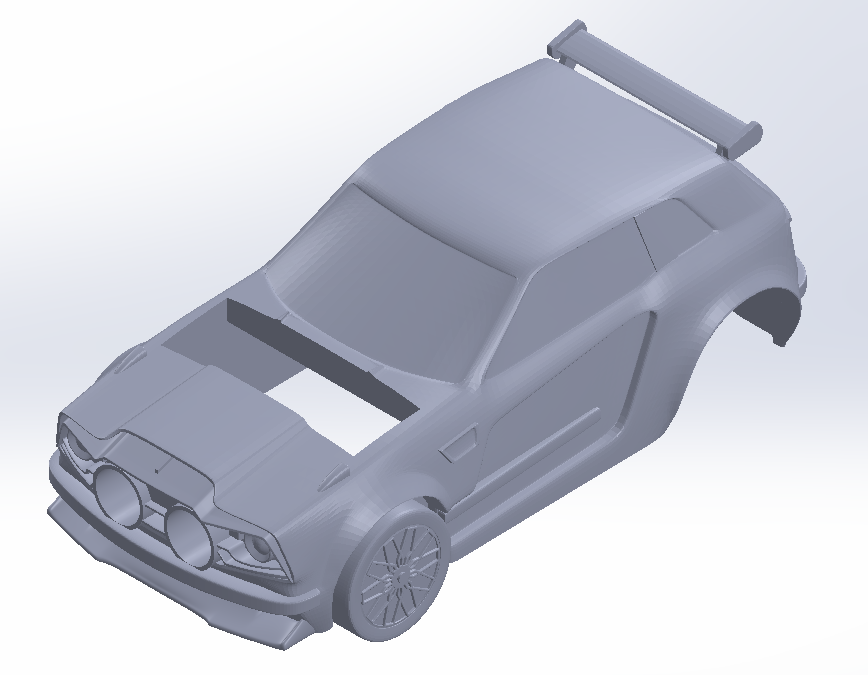
\includegraphics[width=1\textwidth]{solidworks/solidworks1.png}
    	\label{fig:Vue principale conception 3D}
    \end{minipage}
    \hfill%
    \begin{minipage}[c]{.46\linewidth}
        \centering
        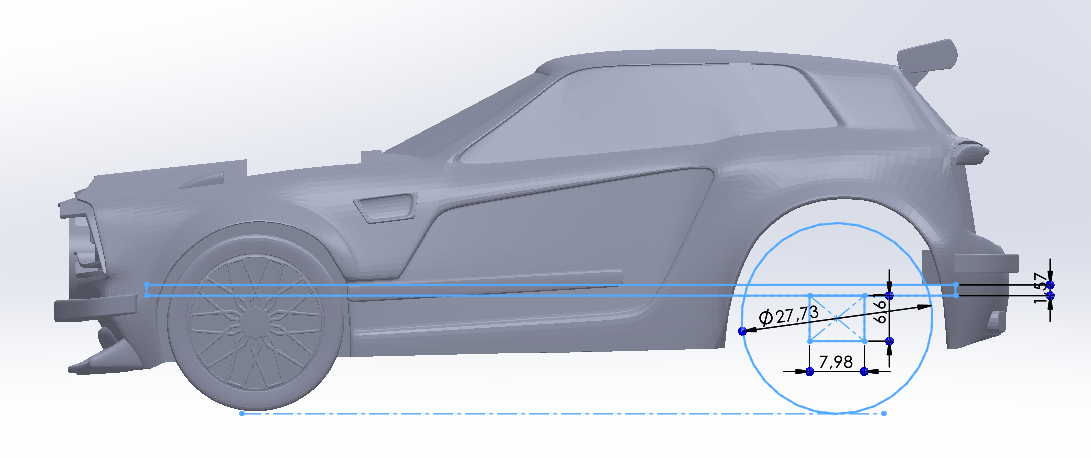
\includegraphics[width=1\textwidth]{solidworks/solidworks3.png}
    	\label{fig:Vue de côté conception 3D}
    \end{minipage}
    \begin{minipage}[c]{.46\linewidth}
        \centering
        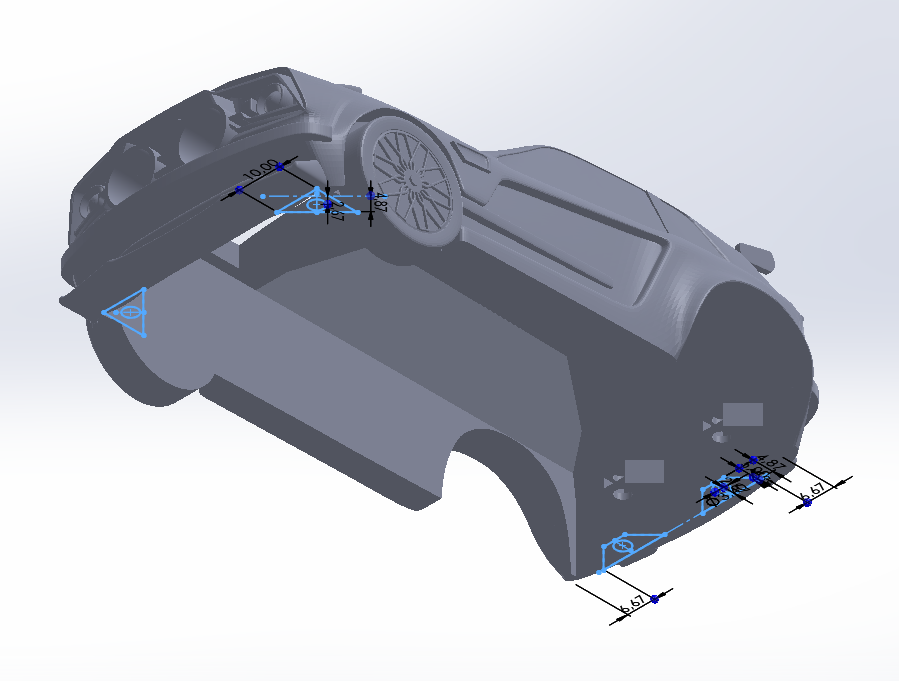
\includegraphics[width=1\textwidth]{solidworks/solidworks2.png}
    	\label{fig:Vue du dessous 2 conception 3D}
    \end{minipage}
    \hfill%
    \begin{minipage}[c]{.46\linewidth}
        \centering
       	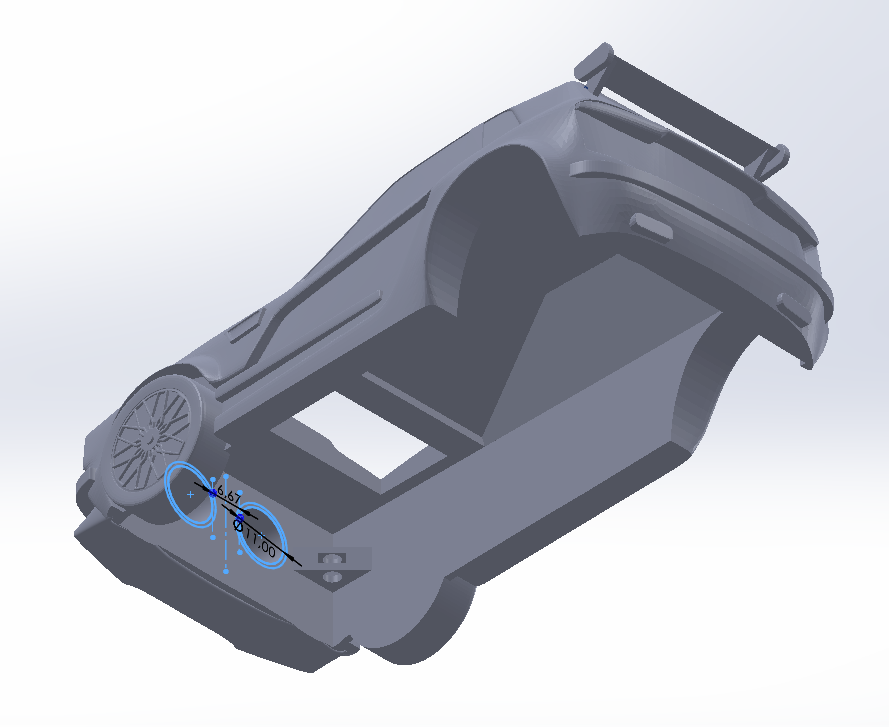
\includegraphics[width=1\textwidth]{solidworks/solidworks4.png}
    	\label{fig:Vue du dessous conception 3D}
    \end{minipage}
    \caption{Captures d'écran de la conception 3D sous SolidWorks}
\end{figure}

\newpage